\documentclass{standalone}
\usepackage{tikz}
\usetikzlibrary{calc}
\usetikzlibrary{decorations.markings}


\begin{document}
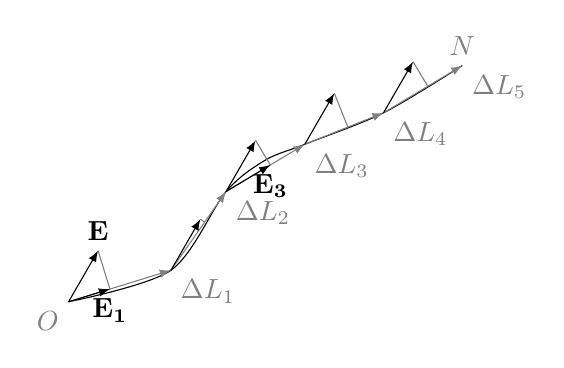
\begin{tikzpicture}[decoration={
  markings,
  mark=at position 0.5 with {\arrow[gray]{>}}}
]
%\draw[gray,thick] grid (5,3);
%\draw[gray,thin,step=0.2] grid (5,3);

%smooth curve
\draw plot[smooth] coordinates {(0,0) (1.3,0.4) (2,1.4) (2.5,1.8) (3,2) (4,2.4) (5,3)};
%small sections
\draw[gray,-latex] (0,0) node [below left]{$O$}-- (1.3,0.4) node[below right]{$\Delta L_1$};
\draw[gray,-latex] (1.3,0.4) --(2,1.4)node[below right]{$\Delta L_2$};
\draw[gray,-latex] (2,1.4) --(3,2)node[below right]{$\Delta L_3$};
\draw[gray,-latex]  (3,2) --(4,2.4)node[below right]{$\Delta L_4$};
\draw[gray,-latex] (4,2.4) --(5,3)node[below right]{$\Delta L_5$} node [above]{$N$};
%
%field
\draw[-latex] (0,0)--(60:0.75cm) node[above] {$\bf{E}$};
\draw[-latex](1.3,0.4)--+(60:0.75cm);
\draw[-latex] (2,1.4)--+(60:0.75cm);
\draw[-latex] (3,2)--+(60:0.75cm) ;
\draw[-latex] (4,2.4)--+(60:0.75cm);
%field components vertical drops
\coordinate (K1) at ($(0,0)+(60:0.75cm)$);
\coordinate (K2) at ($(1.3,0.4)+(60:0.75cm)$);
\coordinate (K3) at ($(2,1.4)+(60:0.75cm)$);
\coordinate (K4) at ($(3,2)+(60:0.75cm)$);
\coordinate (K5) at ($ (4,2.4)+(60:0.75cm)$);

\draw[gray] (K1)--($(0,0)!(K1)! (1.3,0.4)$);
\draw[gray] (K2)--($(1.3,0.4) !(K2)!(2,1.4)$);
\draw[gray] (K3)--($(2,1.4) !(K3)!(3,2)$);
\draw[gray] (K4)--($(3,2)!(K4)! (4,2.4)$);
\draw[gray] (K5)--($ (4,2.4) !(K5)!(5,3)$);
%field components
\draw[-latex] (0,0)--($(0,0)!(K1)! (1.3,0.4)$) node [below] {$\bf{E}_1$};
\draw[-latex] (2,1.4)--($(2,1.4) !(K3)!(3,2)$) node [below] {$\bf{E}_3$};
\end{tikzpicture}

\end{document}
